\documentclass[10pt]{article}

\pagestyle{empty}

\setlength{\textheight}{250mm}
\setlength{\textwidth}{180mm}
\setlength{\oddsidemargin}{-8mm}
\setlength{\topmargin}{-1.5cm}

\usepackage{amsmath}
\usepackage{amsthm}
\usepackage{psfrag}
\usepackage{graphicx}
\usepackage{bm}
\usepackage{mathrsfs}
\usepackage{icomma} % pacchetto per limitare lo spazio standard posto dopo la virgola in caso che la virgola sia tra cifre
\usepackage{amsfonts} % amplia i caratteri matematici disponibili
\usepackage{amssymb}
%\usepackage{wrapfig}
\usepackage{empheq}

\usepackage{epstopdf}
\usepackage[utf8x]{inputenc}
\usepackage{ifthen}

\usepackage{caption}

\usepackage[italian]{babel}
%\usepackage[latin1]{inputenc}

\usepackage{subfig}

\usepackage{pgfplots}
\pgfplotsset{compat=1.9}

%\include{def}

%\newcommand{\kg}{\textrm{kg}}
%\newcommand{\K}{\textrm{K}}
%\newcommand{\m} {\textrm{m}}
%\newcommand{\dm}{\textrm{dm}}
%\newcommand{\cm}{\textrm{cm}}
%\newcommand{\mm}{\textrm{mm}}
%\newcommand{\s} {\textrm{s}}
%\newcommand{\N} {\textrm{N}}
%\renewcommand{\Pa}{\textrm{Pa}}
%\newtheorem{exerciseS}{Esercizio}

\def \flagSect{0} % 1    : numerazione
		  % else : niente
%\newcommand{\taitol}[1]  % stile titolo
%{
%%{\textit{#1}}
%{#1}
%}
\def \soluzione{Soluzione}
\def \partePrima{Concetti. }
\def \parteSeconda{Svolgimento. }
%\def \parteTerza{}
\newcommand{\sol}{\subsubsection*{\soluzione}}
\newcommand{\partone}{\ \ \ \ \ \textbf{\partePrima}}
\newcommand{\parttwo}{\vspace{0.2cm}\textbf{\parteSeconda}}

\ifnum\flagSect=1
\newtheorem{esercizio}{Esercizio}%[section]
\else
\newtheorem*{esercizio}{Esercizio}
\fi

\newtheorem*{teorema}{Teorema}
\newtheorem*{lemma}{Lemma}

% ###########################################################
%\def \flagSect{0} % 1    : numerazione
		  % else : niente
%\newcommand{\taitol}[1]  % stile titolo
%{
%%{\textit{#1}}
%{#1}
%}
\def \soluzione{Soluzione}
\def \partePrima{Concetti. }
\def \parteSeconda{Svolgimento. }
%\def \parteTerza{}
\newcommand{\sol}{\subsubsection*{\soluzione}}
\newcommand{\partone}{\ \ \ \ \ \textbf{\partePrima}}
\newcommand{\parttwo}{\vspace{0.2cm}\textbf{\parteSeconda}}

\ifnum\flagSect=1
\newtheorem{esercizio}{Esercizio}%[section]
\else
\newtheorem*{esercizio}{Esercizio}
\fi

\newtheorem*{teorema}{Teorema}
\newtheorem*{lemma}{Lemma}

% ###########################################################
%\def \flagSect{0} % 1    : numerazione
		  % else : niente
%\newcommand{\taitol}[1]  % stile titolo
%{
%%{\textit{#1}}
%{#1}
%}
\def \soluzione{Soluzione}
\def \partePrima{Concetti. }
\def \parteSeconda{Svolgimento. }
%\def \parteTerza{}
\newcommand{\sol}{\subsubsection*{\soluzione}}
\newcommand{\partone}{\ \ \ \ \ \textbf{\partePrima}}
\newcommand{\parttwo}{\vspace{0.2cm}\textbf{\parteSeconda}}

\ifnum\flagSect=1
\newtheorem{esercizio}{Esercizio}%[section]
\else
\newtheorem*{esercizio}{Esercizio}
\fi

\newtheorem*{teorema}{Teorema}
\newtheorem*{lemma}{Lemma}

% ###########################################################
%\input{logicNumb}
%\newcommand{\sectionIf}[2]
%{
%   \ifthenelse{\equal{#1}{1}}
%              {\subsection{#2}}{\subsection*{#2}}
%}
% ###########################################################

%\newcommand{\sectionIf}[2]
%{
%   \ifthenelse{\equal{#1}{1}}
%              {\subsection{#2}}{\subsection*{#2}}
%}
% ###########################################################

%\newcommand{\sectionIf}[2]
%{
%   \ifthenelse{\equal{#1}{1}}
%              {\subsection{#2}}{\subsection*{#2}}
%}
% ###########################################################


\begin{document}

\begin{center}
\textbf{Esercizi per il corso di Fluidodinamica} 
\medskip
\end{center}


\noindent
\begin{tabular}{cc}
\begin{minipage}[b]{0.60\textwidth}
\begin{exerciseS}[Efflusso da serbatoio]
Si consideri il serbatoio rappresentato in figura, $D=2\ m$, 
$H=4.4\ m$ al cui interno \`{e} contenuta acqua, 
$\overline{\rho}=999\,{kg/m^3}$. 
Supponendo il fluido non viscoso, determinare la velocit\`{a} di 
efflusso del fluido dall'ugello del serbatoio, $h=0.4\ m$ 
e $d = 1\ cm$, e la sua portata, sia in massa sia in volume.

($U = 8.86\ m/s$, $Q=6.96\, 10^{-4}\ m^3/s$, $\overline{Q}=0.695\ kg/s$)
\end{exerciseS}
\end{minipage}
&
\begin{minipage}{0.35\textwidth}
   \begin{center}
   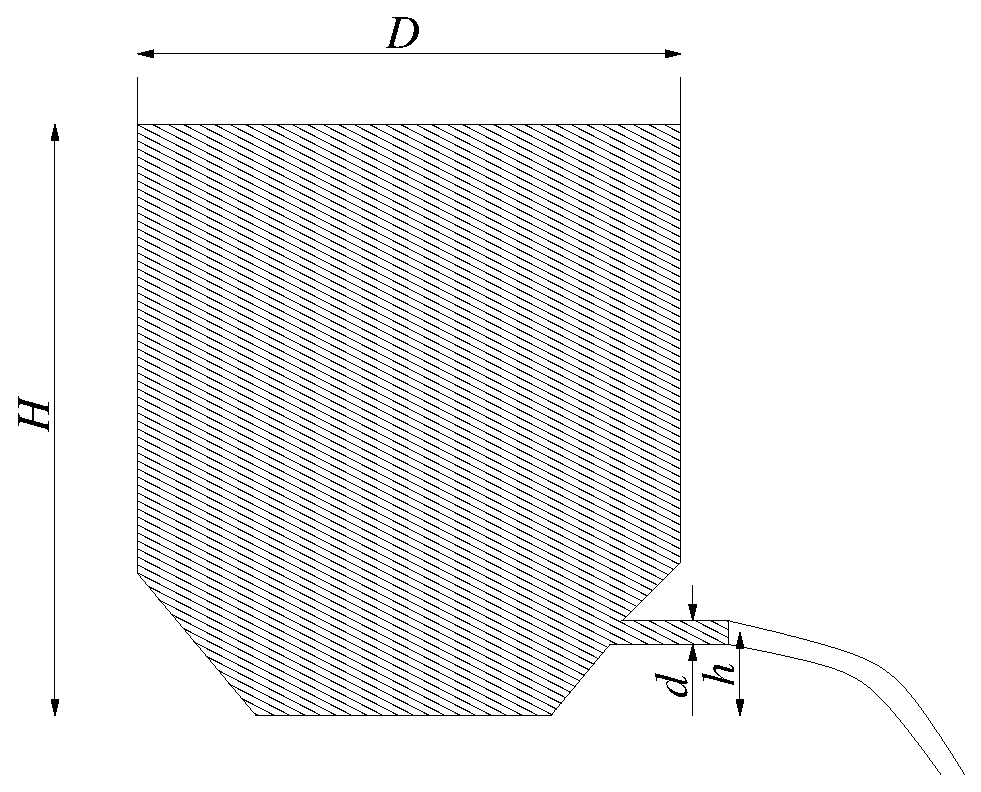
\includegraphics[width=0.90\textwidth]{./fig/serbatoio.eps}
   \end{center}
\end{minipage}
\end{tabular}

\sol

\partone
 Teorema di Bernoulli, nel caso incomprimibile, non viscoso, "stazionario" (da come è
 fatto il disegno, il livello del serbatorio sembra diminuire...assumiamo che così non sia), con forze che ammettono
potenziale e dominio semplicemente connesso.
Se si fa l'ipotesi che il flusso sia irrotazionale sulla sezione di ingresso, nel caso non viscoso, 
si mantiene irrotazionale ovunque (equazione della vorticità).
\begin{equation}
  \frac{D \bm{\omega}}{Dt} = (\bm{\omega} \cdot \bm{\nabla}) \bm{u}
\end{equation}

Si può quindi scrivere il teorema di Bernoulli nella forma:
\begin{equation}
  \frac{P}{\rho} + \frac{|\bm{u}|^2}{2} + gh = \text{cost}
\end{equation}

\parttwo
 Il problema si risolve mettendo a sistema il teorema di Bernoulli (opportunamente
semplificato; vedi sopra) con il bilancio integrale di massa. Si ipotizza che sulle due sezioni agisca la stessa pressione esterna.

\begin{equation}
\begin{cases}
  A_1 u_1 = A_2 u_2 & (massa) \\
  \frac{u_1^2}{2} + g h_1 = \frac{u_2^2}{2} + g h_2 & (Bernoulli)
\end{cases}
\end{equation}

Svolgendo i passaggi, ricordando che le superfici sono circolari, risulta:
\begin{equation}
  u_2 = \sqrt{\frac{2 g (h_1-h_2)}{1-\displaystyle\left(\frac{d_2}{d_1}\right)^4}}
\end{equation}

Si calcolano poi le portate volumetriche e di massa.
\begin{equation}
\begin{aligned}
  & Q = A_2 u_2 \\
  & \dot{m} = \rho Q
\end{aligned}
\end{equation}

%%%%%%%%%%%%%%%%%%%%%%%%%%%%%%%%%%%%%%%%%%%%%%%%%%%%%%%%%%%%%%%%%%

%%%%%%%%%%%%%%%%%%%%%%%%%%%%%%%%%%%%%%%%%%%%%%%%%%%%%%%%%%%%%%%%%%

%%%%%%%%%%%%%%%%%%%%%%%%%%%%%%%%%%%%%%%%%%%%%%%%%%%%%%%%%%%%%%%%%%


%%%%%%%%%%%%%%%%%%%%%%%%%%%%%%%%%%%%%%%%%%%%%%%%%%%%%%%%%%%%%%%%%%

%%%%%%%%%%%%%%%%%%%%%%%%%%%%%%%%%%%%%%%%%%%%%%%%%%%%%%%%%%%%%%%%%%
%%%%%%%%%%%%%%%%%%%%%%%%%%%%%%%%%%%%%%%%%%%%%%%%%%%%%%%%%%%%%%%%%%

\end{document}
